\newpage
\hypertarget{checkCard tex}{}
\subsection{Implementing check}
\texHeader
 
\begin{itemize}
   
\item[$\blacktriangleright$] In this SDM, guess assertion, card promotion, and card penalization must each be implemented as patterns. Given that every
action is determined as the result of a conditional statement, we need an \emph{if/else} construct.

\item[$\blacktriangleright$] In the \texttt{check} method, create the basic \emph{if/else} construct with three patterns, as illustrated in
Fig.~\ref{eclipse:checkDec}. Our auto completion feature includes a template for this.

\vspace{0.5cm}

\begin{figure}[htbp]
\begin{center}
  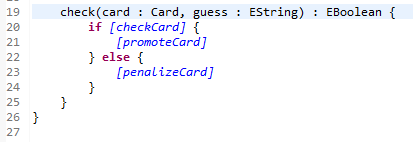
\includegraphics[width=0.65\textwidth]{eclipse_checkCardMethod}
  \caption{An if/else construct in \texttt{check}}
  \label{eclipse:checkDec}
\end{center}
\end{figure} 

\item[$\blacktriangleright$] Upon saving, use the ``Quick Fix'' wizard again to generate the required pattern files. Your package explorer should now resemble
Fig.~\ref{eclipse:checkPatternsExplorer}.

\begin{figure}[htbp]
\begin{center}
  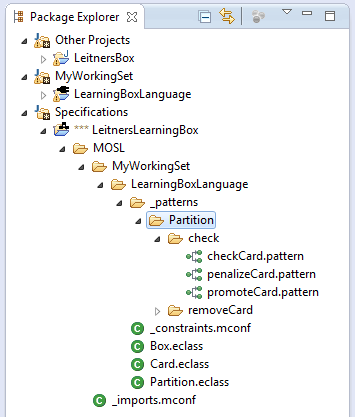
\includegraphics[width=0.55\textwidth]{eclipse_checkPackageExplorer}
  \caption{Project directory after creating patterns}
  \label{eclipse:checkPatternsExplorer}
\end{center}
\end{figure} 

\item[$\blacktriangleright$] Open the \texttt{checkCard} pattern. In order to validate the user's guess, we need to establish an \emph{attribute constraint}
between the \texttt{face} attribute of the current \texttt{card}, and the primitive \texttt{EString} parameter, \texttt{guess}. 

\item[$\blacktriangleright$] As done in Java, referencing the \texttt{face} of a card is done in MOSL via the `dot' operator, so begin the statement with
\texttt{card.face}

\item[$\blacktriangleright$] Attribute constraints have similar operators as Java comparators, so we'll want to use \texttt{`=='} to equate the
values.\footnote{See the \hyperlink{quickRef}{Quick Reference} at the end of this part for a listing of all operators}

\item[$\blacktriangleright$] The tricky part of the overall statement is referencing the parameter value. Given that we have not created an object variable,
we'll need to use another expression type, \texttt{ParameterExpression}\define{ParameterExpression}, to access it. This type exclusively refers to parameter
values, and its syntax is as follows:
\syntax{parameter\_expression := `\$'ID \\
\\
With:\\
ID := STRING}

\item[$\blacktriangleright$] Thus, the complete attribute constraint statement is: \syntax{card.face == \$guess} Your pattern should now resemble
Fig.~\ref{eclipse:checkPattern}.

\vspace{0.5cm}

\begin{figure}[htbp]
\begin{center}
  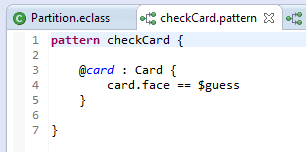
\includegraphics[width=0.5\textwidth]{eclipse_checkPattern}
  \caption{Completed \texttt{checkCard} pattern}
  \label{eclipse:checkPattern}
\end{center}
\end{figure} 

\item[$\blacktriangleright$] Now let's specify the \texttt{promoteCard} pattern. It requires three object variables: the current partition (\texttt{this}),
the card to be promoted, and the partition the card will move to. Open and edit so that it resembles Fig.~\ref{eclipse:promoteCardPattern}.

\item[$\blacktriangleright$] Given that \texttt{this} is bound while \texttt{next} partition is free, we need to establish a reference link between the
\texttt{box} and partition. This will allow the card to be moved around. Create an \emph{outgoing link variable}, \texttt{next},  with target object variable
\texttt{nextPartition}. Your file should now resemble Fig.~\ref{eclipse:promoteThisRule}.

\begin{figure}[htbp]
\begin{center}
  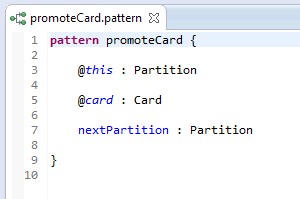
\includegraphics[width=0.5\textwidth]{eclipse_promoteCardPattern}
  \caption{Object variables for promoting a card}
  \label{eclipse:promoteCardPattern}
\end{center}
\end{figure} 

\begin{figure}[htbp]
\begin{center}
  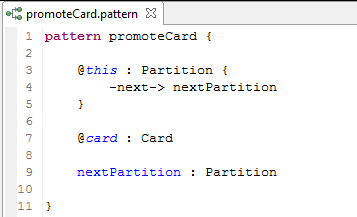
\includegraphics[width=0.5\textwidth]{eclipse_promoteCardThisRule}
  \caption{The \texttt{@this} object variable}
  \label{eclipse:promoteThisRule}
\end{center}
\end{figure} 

\item[$\blacktriangleright$] Finally, let's update the \texttt{cardContainer} reference of \texttt{card}. Simply delete the link to \texttt{this}, and create
a new link to \texttt{nextPartition}.\footnote{There are several different ways you could have implemented this movement, such as updating the link from
\texttt{nextPartition} to \texttt{card}.} Your pattern is now complete.

\vspace{0.5cm}

\item[$\blacktriangleright$] Compare the differences between the \texttt{promoteCard} and \texttt{penalizeCard} concepts. They both do the exact same thing,
except the destination partition is different. Knowing this, try to complete \texttt{penalizeCard} entirely on your own. Your workspace should come to
resemble Fig.~\ref{eclipse:completedPatterns}.

\newpage

\begin{figure}[htbp]
\begin{center}
  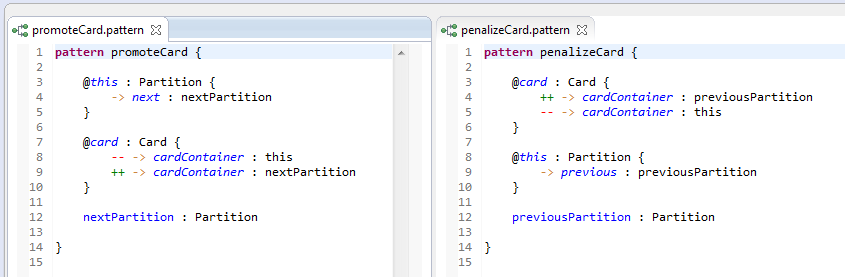
\includegraphics[width=\textwidth]{eclipse_movementPatternsCompleted}
  \caption{Both movement patterns completed}
  \label{eclipse:completedPatterns}
\end{center}
\end{figure}

\item[$\blacktriangleright$] Did you notice that the order of the \texttt{this} and \texttt{card} object variable scopes are reversed in the figures above?
In general, it doesn't matter in which order object or variables are specified in patterns. Everything just needs to be correctly stated. 

\item[$\blacktriangleright$] We nearly forgot to complete the control flow! We have specified the assertion and card movements, but we haven't returned a
\texttt{EBoolean} result as the method requires.  We'll need to implement a new expression type, a \emph{LiteralExpression}\define{LiteralExpression}. This
type can be used to specify arbitrary text, but should really only be used for true literals like 42, ``foo'' or \texttt{true}. The syntax for any LiteralExpression
is simply:
\syntax{LiteralExpression := boolean\_literal | integer\_literal | any\_literal \\
\\
With:\\
boolean\_literal := true, false\\
integer\_literal := [`+' | `-'] ( `1' |\ldots| `9' ) \\
any\_literal := STRING\\
}

\vspace{0.5cm}

\item[$\blacktriangleright$] Knowing this, and that \texttt{guess} was successful
when the card was promoted, return \texttt{true} beneath \texttt{promoteCard}. If it was penalized, return \texttt{false}. Your \texttt{check} method
should now resemble Fig.\ref{eclipse:finalMethod}.

\vspace{0.5cm}

\item[$\blacktriangleright$] Save and build your metamodel, then try viewing the changes in ``PartitionImpl.Java'' under \texttt{check}. You'll be able to
see the \emph{if/else} construct, as well as the link manipulations. 

\newpage

\begin{figure}[htbp]
\begin{center}
  \includegraphics[width=0.7\textwidth]{eclipse_checkMethodFinal}
  \caption{Completed control flow for \texttt{check}}
  \label{eclipse:finalMethod}
\end{center}
\end{figure}

\item[$\blacktriangleright$] Great job! You have just enabled checking a card with guesses via a new control flow construct, \emph{if/else}, and two patterns
that move the cards appropriately. To see how this SDM is implemented visually, check out Fig.~\ref{ea:sdm_check_finish} for the control flow, and
Figs.~\ref{ea:sdm_check_complete_activity_node} and \ref{ea:sdm_check_complete_penalize} for the movement patterns, all in the previous visual section.

\end{itemize}
 